%-- coding:UTF-8 --
\documentclass{article}

\usepackage[english]{babel}
\usepackage[UTF8]{ctex}

\usepackage[letterpaper,top=2cm,bottom=2cm,left=3cm,right=3cm,marginparwidth=1.75cm]{geometry}

\usepackage{amsmath}
\usepackage{graphicx}
\usepackage[colorlinks=true, allcolors=blue]{hyperref}
\usepackage{booktabs}
\usepackage{tabularx}
\usepackage{multirow}
\usepackage{listings}
\usepackage{minted}
\usepackage{xcolor}

\lstdefinestyle{myStyle}{
    backgroundcolor=\color{gray!10}, % 设定背景颜色
    basicstyle=\ttfamily, % 设置基本字体
%    frame=single, % 添加框架
%    rulecolor=\color{black}, % 框架颜色
    keywordstyle=\color{blue}, % 关键字颜色
    commentstyle=\color{green}, % 注释颜色
    stringstyle=\color{red} % 字符串颜色
}


\title{实验2:shell工具和脚本}
\author{方欣 23020007021}
\date{}

\begin{document}
\maketitle

\url{https://github.com/nixgnaf/SDT_report.github.io}

\section{shell命令实例}
\subsection{目录管理}

\subsubsection{创建目录(mkdir)}
\begin{lstlisting}[style=myStyle]
mkdir [-p] dirName
\end{lstlisting}
参数说明:-p 确保目录名称存在,不存在的就建一个。
\begin{figure}[h]
    \centering
    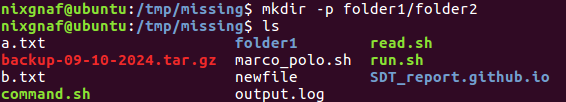
\includegraphics[width=0.5\linewidth]{image8.png}
\end{figure}

\subsubsection{删除目录(rmdir)}
\begin{lstlisting}[style=myStyle]
mkdir [-p] dirName
\end{lstlisting}
-p 是当子目录被删除后使它也成为空目录的话,则顺便一并删除。
\begin{figure}[h]
    \centering
    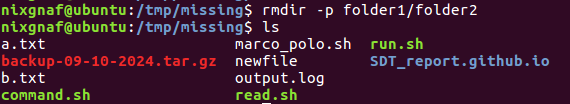
\includegraphics[width=0.5\linewidth]{image9.png}
\end{figure}

\subsubsection{显示工作目录(pwd)}
\begin{lstlisting}[style=myStyle]
pwd [--help][--version]
\end{lstlisting}
执行 pwd 指令可立刻得知您目前所在的工作目录的绝对路径名称。\\
参数说明:\\
--help 在线帮助。
--version 显示版本信息。
\begin{figure}[h]
    \centering
    
\includegraphics[width=0.5\linewidth]{image10.png}
\end{figure}

\subsubsection{显示目录内容(ls)}
\begin{lstlisting}[style=myStyle]
 ls [-alrtAFR] [name...]
\end{lstlisting}
ls命令用于显示指定工作目录下之内容(列出目前工作目录所含的文件及子目录)。\\
参数 :\\
-a 显示所有文件及目录 (. 开头的隐藏文件也会列出)\\
-d 只列出目录(不递归列出目录内的文件)。\\
-l 以长格式显示文件和目录信息,包括权限、所有者、大小、创建时间等\\。
-r 倒序显示文件和目录。\\
-t 将按照修改时间排序,最新的文件在最前面。\\
-A 同 -a ,但不列出 "." (目前目录) 及 ".." (父目录)\\
-F 在列出的文件名称后加一符号;例如可执行档则加 "*", 目录则加 "/"\\
-R 递归显示目录中的所有文件和子目录。
\begin{figure}[h]
    \centering
    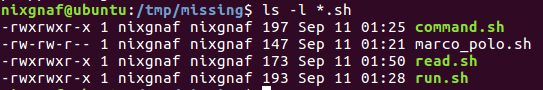
\includegraphics[width=0.5\linewidth]{image11.png}
\end{figure}

\subsubsection{改变当前目录(cd)}
\begin{lstlisting}[style=myStyle]
cd [dirName]
\end{lstlisting}
cd 命令用于改变当前工作目录的命令,切换到指定的路径。\\
若目录名称省略,则变换至使用者的 home 目录 (也就是刚 login 时所在的目录)。\\
另外,~ 也表示为 home 目录 的意思, . 则是表示目前所在的目录, .. 则表示目前目录位置的上一层目录。\\
dirName:要切换的目标目录,可以是相对路径或绝对路径。
\begin{figure}[h]
    \centering
    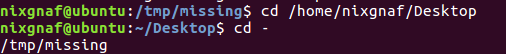
\includegraphics[width=0.5\linewidth]{image12.png}
\end{figure}

\subsubsection{目录重命名(mv)}
\begin{lstlisting}[style=myStyle]
mv [options] source dest
mv [options] source... directory
mv source_file(文件) dest_file(文件)
mv source_file(文件) dest_directory(目录)
mv source_directory(目录) dest_directory(目录)
\end{lstlisting}
将源文件名 source\_file 改为目标文件名 dest\_file\\
将文件 source\_file 移动到目标目录 dest\_directory 中\\
目录名 dest\_directory 已存在,将 source\_directory 移动到目录名 dest\_directory 中;目录名 dest\_directory 不存在则 source\_directory 改名为目录名 dest\_directory\\
参数说明:\\
-b: 当目标文件或目录存在时,在执行覆盖前,会为其创建一个备份。\\
-i: 如果指定移动的源目录或文件与目标的目录或文件同名,则会先询问是否覆盖旧文件,输入 y 表示直接覆盖,输入 n 表示取消该操作。\\
-f: 如果指定移动的源目录或文件与目标的目录或文件同名,不会询问,直接覆盖旧文件。\\
-n: 不要覆盖任何已存在的文件或目录。\\
-u:当源文件比目标文件新或者目标文件不存在时,才执行移动操作。\\
\begin{figure}[h]
    \centering
    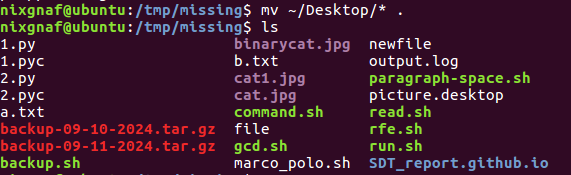
\includegraphics[width=0.5\linewidth]{image13.png}
\end{figure}


\subsubsection{目录拷贝(cp)}
\begin{lstlisting}[style=myStyle]
cp [options] source... dest
\end{lstlisting}
source(源文件)表示要复制的文件或目录的路径,dest(目标文件)表示复制后的文件或目录的路径。\\
参数说明:\\
-a:此选项通常在复制目录时使用,它保留链接、文件属性,并复制目录下的所有内容。其作用等于 dpR 参数组合。\\
-d:复制时保留链接。这里所说的链接相当于 Windows 系统中的快捷方式。\\
-r 或 --recursive:用于复制目录及其所有的子目录和文件,如果要复制目录,需要使用该选项。\\
-i 或 --interactive:在复制前提示确认,如果目标文件已存在,则会询问是否覆盖,回答 y 时目标文件将被覆盖。\\
-u 或 --update:仅复制源文件中更新时间较新的文件。\\
-v 或 --verbose:显示详细的复制过程。\\
-p 或 --preserve:保留源文件的权限、所有者和时间戳信息。\\
-f 或 --force:强制复制,即使目标文件已存在也会覆盖,而且不给出提示。\\
-l:不复制文件,只是生成链接文件。
\begin{figure}[h]
    \centering
    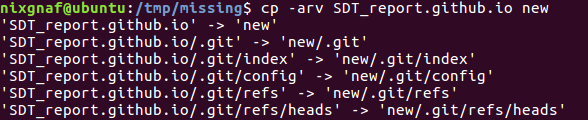
\includegraphics[width=0.5\linewidth]{image14.png}
\end{figure}
\subsection{文件管理}

\subsubsection{新建文件(> FileName/touch FileName/vim FileName)}
\begin{lstlisting}[style=myStyle]
touch [-acfm][-d<日期时间>][-r<参考文件或目录>] [-t<日期时间>]
[--help][--version][文件或目录…]
\end{lstlisting}
touch命令用于修改文件或者目录的时间属性,包括存取时间和更改时间。若文件不存在,系统会建立一个新的文件。\\
参数说明:\\
-a: 改变档案的读取时间记录。\\
-m: 改变档案的修改时间记录。\\
-c: 假如目的档案不存在,不会建立新的档案。与 --no-create 的效果一样。\\
-f: 不使用,是为了与其他 unix 系统的相容性而保留。\\
-r: 使用参考档的时间记录,与 --file 的效果一样。\\
d: 设定时间与日期,可以使用各种不同的格式。\\
t: 设定档案的时间记录,格式与 date 指令相同。\\
--no-create 不会建立新档案。\\
\begin{figure}[h]
    \centering
    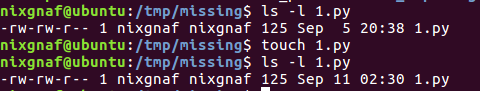
\includegraphics[width=0.5\linewidth]{image15.png}
\end{figure}

\subsubsection{删除文件(rm)}
\begin{lstlisting}[style=myStyle]
rm [options] name...
\end{lstlisting}
参数说明:\\
-i 系统提示是否真要删除该文件.\\
-f 删除文件之前不提示任何确认信息.\\
-r 递归删除目录下所有子目录的内容.\\
\begin{figure}[h]
    \centering
    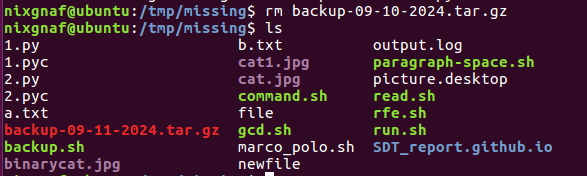
\includegraphics[width=0.5\linewidth]{image16.png}
\end{figure}

\subsubsection{文件链接(ln)}
\begin{lstlisting}[style=myStyle]
 ln [参数][源文件或目录][目标文件或目录]
\end{lstlisting}
 ln命令是一个非常重要命令,它的功能是为某一个文件在另外一个位置建立一个同步的链接。\\
当我们需要在不同的目录,用到相同的文件时,我们不需要在每一个需要的目录下都放一个必须相同的文件,我们只要在某个固定的目录,放上该文件,然后在 其它的目录下用ln命令链接(link)它就可以,不必重复的占用磁盘空间。\\
参数说明:\\
--backup[=CONTROL] 备份已存在的目标文件\\
-b 类似 --backup ,但不接受参数\\
-d 允许超级用户制作目录的硬链接\\
-f 强制执行\\
-i 交互模式,文件存在则提示用户是否覆盖\\
-n 把符号链接视为一般目录\\
-s 软链接(符号链接)\\
-v 显示详细的处理过程\\

\begin{figure}[h]
    \centering
    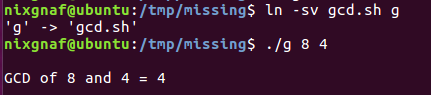
\includegraphics[width=0.5\linewidth]{image17.png}
\end{figure}

\subsubsection{显示文件内容(more/less/cat/head/tail/nl)}
\begin{lstlisting}[style=myStyle]
more [-dlfpcsu] [-num] [+/pattern] [+linenum] [fileNames..]
less [参数] 文件 
cat [选项] [文件]
head [参数] [文件]
tail [参数] [文件]  
\end{lstlisting}
以一页一页的形式显示,更方便使用者逐页阅读,而最基本的指令就是按空白键(space)就往下一页显示,按 b 键就会往回(back)一页显示,而且还有搜寻字串的功能(与 vi 相似),使用中的说明文件,请按 h 。\\
less 与 more 类似,less 可以随意浏览文件,支持翻页和搜索,支持向上翻页和向下翻页。\\

\noindent cat 命令用于连接文件并打印到标准输出设备上,它的主要作用是用于查看和连接文件。\\
参数说明:\\
-n:显示行号,会在输出的每一行前加上行号。\\
-b:显示行号,但只对非空行进行编号。\\
-s:压缩连续的空行,只显示一个空行。\\
-E:在每一行的末尾显示 \$ 符号。\\
-T:将 Tab 字符显示为 \^I。\\
-v:显示一些非打印字符。\\
使用说明:\\
显示文件内容:cat filename 会将指定文件的内容输出到终端上。\\
连接文件:cat file1 file2 > combined\_file 可以将 file1 和 file2 的内容连接起来,并将结果输出到 combined\_file 中。\\
创建文件:可以使用 cat 命令来创建文件,例如 cat > filename,然后你可以输入文本,按 Ctrl+D 来保存并退出。\\
在终端显示文件:可以将 cat 与管道(|)结合使用,用来显示其他命令的输出,例如 ls -l | cat 会将 ls -l 的输出通过 cat 打印到终端上。\\

\noindent head 命令可用于查看文件的开头部分的内容,有一个常用的参数 -n 用于显示行数,默认为 10,即显示 10 行的内容。\\
参数说明:\\
-q 隐藏文件名\\
-v 显示文件名\\
-c<数目> 显示的字节数。\\
-n<行数> 显示的行数。\\

\noindent tail 命令可用于查看文件的内容,有一个常用的参数 -f 常用于查阅正在改变的日志文件。\\
tail -f filename 会把 filename 文件里的最尾部的内容显示在屏幕上,并且不断刷新,只要 filename 更新就可以看到最新的文件内容。\\
参数说明:\\
-f 循环读取\\
-q 不显示处理信息\\
-v 显示详细的处理信息\\
-c<数目> 显示的字节数\\
-n<行数> 显示文件的尾部 n 行内容\\
--pid=PID 与-f合用,表示在进程ID,PID死掉之后结束\\
-q, --quiet, --silent 从不输出给出文件名的首部\\
-s, --sleep-interval=S 与-f合用,表示在每次反复的间隔休眠S秒\\
\begin{figure}[h]
    \centering
    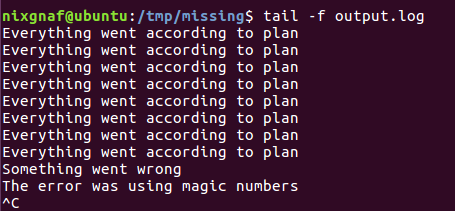
\includegraphics[width=0.5\linewidth]{image18.png}
\end{figure}

\subsubsection{文件查找(find)}
\begin{lstlisting}[style=myStyle]
find [路径] [匹配条件] [动作]
\end{lstlisting}
find 命令用于在指定目录下查找文件和目录。\\
它可以使用不同的选项来过滤和限制查找的结果。\\
参数说明 :\\
路径 是要查找的目录路径,可以是一个目录或文件名,也可以是多个路径,多个路径之间用空格分隔,如果未指定路径,则默认为当前目录。\\
expression 是可选参数,用于指定查找的条件,可以是文件名、文件类型、文件大小等等。\\
匹配条件 中可使用的选项有二三十个之多,以下列出最常用的部份:\\
-name pattern:按文件名查找,支持使用通配符 * 和 ?。\\
-type type:按文件类型查找,可以是 f(普通文件)、d(目录)、l(符号链接)等。\\
-size [+-]size[cwbkMG]:按文件大小查找,支持使用 + 或 - 表示大于或小于指定大小,单位可以是 c(字节)、w(字数)、b(块数)、k(KB)、M(MB)或 G(GB)。\\
-mtime days:按修改时间查找,支持使用 + 或 - 表示在指定天数前或后,days 是一个整数表示天数。\\
-user username:按文件所有者查找。\\
-group groupname:按文件所属组查找。\\
动作: 可选的,用于对匹配到的文件执行操作,比如删除、复制等。\\
\begin{figure}[h]
    \centering
    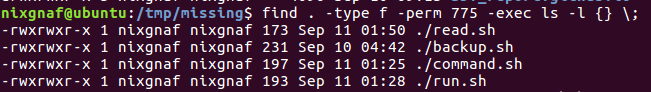
\includegraphics[width=0.5\linewidth]{image19.png}
\end{figure}

\subsubsection{文件内容查找(grep)}
\begin{lstlisting}[style=myStyle]
grep [options] pattern [files]
\end{lstlisting}
grep (global regular expression) 命令用于查找文件里符合条件的字符串或正则表达式。\\
grep 指令用于查找内容包含指定的范本样式的文件,如果发现某文件的内容符合所指定的范本样式,预设 grep 指令会把含有范本样式的那一列显示出来。若不指定任何文件名称,或是所给予的文件名为 -,则 grep 指令会从标准输入设备读取数据。\\
pattern - 表示要查找的字符串或正则表达式。\\
files - 表示要查找的文件名,可以同时查找多个文件,如果省略 files 参数,则默认从标准输入中读取数据。\\
常用参数:\\
-i:忽略大小写进行匹配。\\
-v:反向查找,只打印不匹配的行。\\
-n:显示匹配行的行号。\\
-r:递归查找子目录中的文件。\\
-l:只打印匹配的文件名。\\
-c:只打印匹配的行数。\\
\begin{figure}[h]
    \centering
    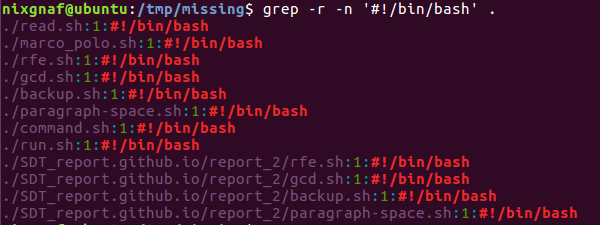
\includegraphics[width=0.5\linewidth]{image20.png}
\end{figure}

\subsection{权限管理}

\subsubsection{改变文件/目录的权限(chmod)}
\begin{lstlisting}[style=myStyle]
chmod [-cfvR] [--help] [--version] mode file...
(mode:)[ugoa...][[+-=][rwxX]...][,...]
\end{lstlisting}
Linux/Unix 的文件调用权限分为三级 : 文件所有者(Owner)、用户组(Group)、其它用户(Other Users)。\\
u 表示该文件的拥有者,g 表示与该文件的拥有者属于同一个群体(group)者,o 表示其他以外的人,a 表示这三者皆是。\\
+ 表示增加权限、- 表示取消权限、= 表示唯一设定权限。\\
r 表示可读取,w 表示可写入,x 表示可执行,X 表示只有当该文件是个子目录或者该文件已经被设定过为可执行。\\
其他参数说明:\\
-c : 若该文件权限确实已经更改,才显示其更改动作\\
-f : 若该文件权限无法被更改也不要显示错误讯息\\
-v : 显示权限变更的详细资料\\
-R : 对目前目录下的所有文件与子目录进行相同的权限变更(即以递归的方式逐个变更)\\
\begin{figure}[h]
    \centering
    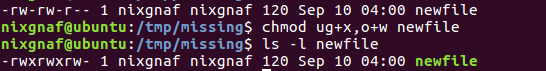
\includegraphics[width=0.5\linewidth]{image21.png}
\end{figure}

\subsubsection{改变文件/目录的属主/属组(chown/chgrp)}
\begin{lstlisting}[style=myStyle]
chown [-cfhvR] [--help] [--version] user[:group] file...
chgrp [-cfhRv][--help][--version][所属群组][文件或目录...]
\end{lstlisting}
chown 命令用于设置文件所有者和文件关联组的命令。\\
Linux chgrp 命令用于变更文件或目录的所属群组。
与 chown 命令不同,chgrp 允许普通用户改变文件所属的组,只要该用户是该组的一员。\\
参数说明:\\
user : 新的文件拥有者的使用者 ID\\
group : 新的文件拥有者的使用者组(group)\\
-c : 显示更改的部分的信息\\
-f : 忽略错误信息\\
-h :修复符号链接\\
-v : 显示详细的处理信息\\
-R : 处理指定目录以及其子目录下的所有文件\\
\begin{figure}[h]
    \centering
    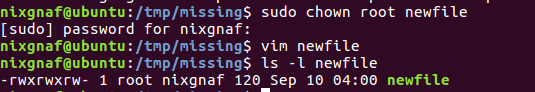
\includegraphics[width=0.5\linewidth]{image22.png}
\end{figure}

\newpage
\subsection{递归查找文件并压缩}
本命令组合的作用是将当前目录及其子目录中所有 .html 文件打包成一个名为 html.zip 的压缩文件。\\
find . -type f -name "*.html":\\
查找当前目录及其子目录中所有扩展名为 .html 的文件。\\
xargs -d '\\n' tar -cvzf html.zip:\\
xargs -d '\\n':将 find 命令输出的每个文件名作为 tar 命令的参数。-d '\\n' 表示使用换行符作为分隔符。\\
tar -cvzf html.zip:将文件打包并压缩成 html.zip。-c 创建新归档,-v 显示过程,-z 使用 gzip 压缩,-f 指定输出文件名。\\
\begin{figure}[h]
    \centering
    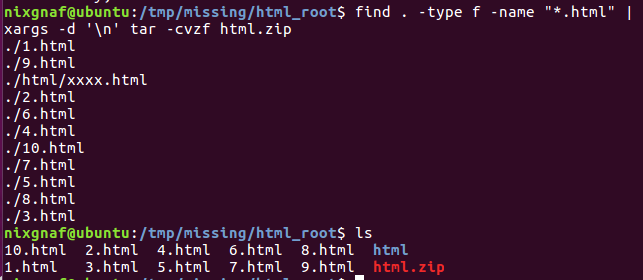
\includegraphics[width=0.5\linewidth]{image23.png}
\end{figure}

\subsection{按照最近使用时间列出文件}
本命令组合的作用是列出在当前目录及其子目录中,在过去 60 分钟内修改过的所有文件,并按修改时间排序,最新的文件排在最前面。\\
find . -type f -mmin -60 -print0:\\
find .:在当前目录及其子目录中查找。\\
-type f:只查找文件(不包括目录)。\\
-mmin -60:查找过去 60 分钟内被修改过的文件。\\
-print0:以 null 字符 (\\0) 分隔输出的文件名,以处理包含空格或特殊字符的文件名。\\
xargs -0 ls -lt:\\
xargs -0:将 find 输出的 null 分隔的文件名传递给 ls 命令。\\
ls -lt:列出这些文件的详细信息,并按修改时间排序,最新修改的文件排在最前面。\\
\begin{figure}[h]
    \centering
    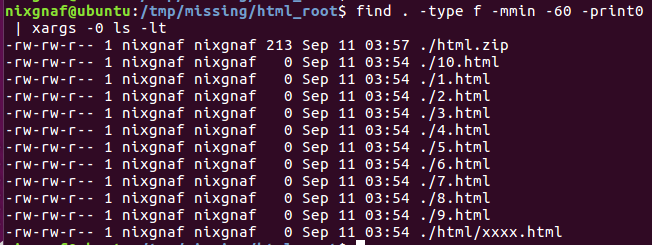
\includegraphics[width=0.5\linewidth]{image24.png}
\end{figure}

\section{脚本实例}

\subsection{文本文件的段间添加空行}
\lstinputlisting[style=myStyle]{paragraph-space.sh}
\begin{figure}[h]
    \centering
    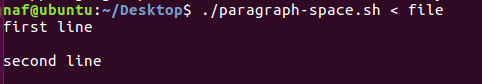
\includegraphics[width=0.5\linewidth]{image6.png}
\end{figure}

\subsection{代码块和I/O重定向}
\lstinputlisting[style=myStyle]{read.sh}

\begin{figure}[h]
    \centering
    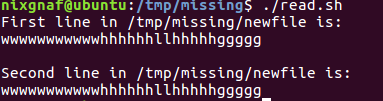
\includegraphics[width=0.5\linewidth]{image1.png}
\end{figure}

\subsection{工作目录的保存与恢复}
\lstinputlisting[style=myStyle]{marco_polo.sh}
\begin{figure}[h]
    \centering
    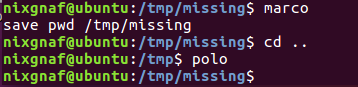
\includegraphics[width=0.5\linewidth]{image2.png}
\end{figure}

\subsection{报告脚本出错前运行次数}
\lstinputlisting[style=myStyle]{command.sh}
\lstinputlisting[style=myStyle]{run.sh}

\begin{figure}[h]
    \centering
    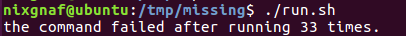
\includegraphics[width=0.5\linewidth]{image3.png}
\end{figure}

\subsection{备份最后一天所修改的文件}
\lstinputlisting[style=myStyle]{backup.sh}
\begin{figure}[h]
    \centering
    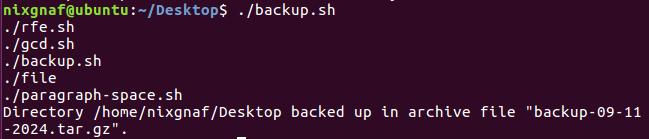
\includegraphics[width=0.5\linewidth]{image7.png}
\end{figure}

\subsection{最大公约数}
\lstinputlisting[style=myStyle]{gcd.sh}
\begin{figure}[h]
    \centering
    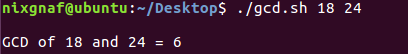
\includegraphics[width=0.5\linewidth]{image4.png}
\end{figure}

\subsection{重命名文件拓展名}
\lstinputlisting[style=myStyle]{rfe.sh}
\begin{figure}[h]
    \centering
    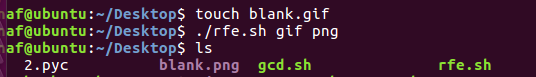
\includegraphics[width=0.5\linewidth]{image5.png}
\end{figure}

\section{数据整理}
\subsection{统计words文件 (/usr/share/dict/words) 中包含至少三个a 且不以's 结尾的单词个数}
\noindent cat /usr/share/dict/words:显示字典文件中的所有单词。\\
tr "[:upper:]" "[:lower:]":将所有单词转换为小写。
grep -E "\^([\^a]*a){3}.*\$":匹配含有至少三个字母 "a" 的单词。\\
grep -v "'s\$":排除以 "'s" 结尾的单词(例如 "cats")。\\
wc -l:计算符合条件的单词数量。\\
\begin{figure}[h]
    \centering
    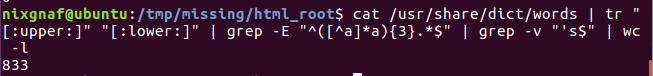
\includegraphics[width=0.5\linewidth]{image25.png}
\end{figure}

这些单词中,出现频率前三的末尾两个字母是什么? \\
sed -E "s/.*([a-z]{2})\$/\textbackslash1/":使用扩展正则表达式将每个单词转换为其最后两个字母。\\
s/.*([a-z]{2})\$/\textbackslash1/ 的意思是:\\
.* 匹配任意字符。\\
([a-z]{2})\$ 捕获字符串的最后两个字母。\\
\textbackslash1 是对捕获的最后两个字母的引用,即替换为这两个字母。\\
sort:将结果按字母顺序排序。
uniq -c:统计每个唯一的结果出现的次数。
sort(第二次):按出现次数对结果进行排序。
tail -n3:显示出现次数最多的最后三个结果
\begin{figure}[h]
    \centering
    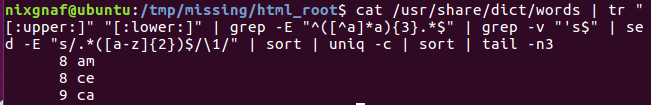
\includegraphics[width=0.5\linewidth]{image26.png}
\end{figure}

共存在多少种词尾两字母组合?\\
uniq:去除重复的最后两个字母组合。
\begin{figure}[h]
    \centering
    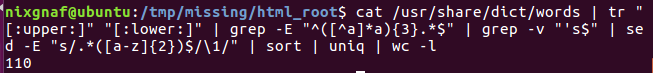
\includegraphics[width=0.5\linewidth]{image27.png}
\end{figure}

\section{结论和心得}

Shell是一种具备特殊功能的程序, 它是介于使用者和 UNIX/Linux 操作系统之核心程序(kernel)间的一个接口。
本质上,shell脚本是命令行命令简单的组合到一个文件里面。Shell基本上是一个命令解释器,类似于DOS下的command.com。它接收用户命令,然后调用相应的应用程序。

通过本次实验,我掌握了shell的基本命令,认识了如何使用常见的 Shell 工具来处理文件和文本数据,并且了解到如何编写 Shell 脚本,通过脚本语言的条件判断、循环结构和函数,能够自动化执行一系列任务。



\end{document}

